\section{Projekte}
\label{section:Projekte}

\subsection{3D Scanner}
\label{section:3dScanner}

\subsubsection{Abh�ngigkeiten}

\begin{itemize}
	\item cg
	\item JOGL
	\item Tinkerforge-Bibliotheken (Unterverzeichnis lib)
\end{itemize}

\subsubsection{Installation}

Zun�chst m�ssen die Projekte cg (Abschnitt \ref{section:cg}) und JOGL (Abschnitt \ref{section:JOGL}) eingerichtet werden. und das Git-Repository (\emph{git.informatik.haw-hamburg.de/srv/git/computergrafik/cg\_3dscanner})  gecloned werden (siehe Abschnitt \ref{section:clone}). Dann wird auch das Projekt \emph{3dscanner} in Eclipse importiert. Als Compiler und f�r die Laufzeitbibliothek muss wegen der Abh�ngigkeit von JOGL Java 1.6 verwendet werden.

Setzen Sie die notwendigen Ressourcenpfade wie unter \ref{section:ressourcen} beschrieben.

\subsubsection{Einrichten des USB-Seriell-Adapters}

Der Treiber (Beispiel Windows XP) befindet sich im Projektverzeichnis unter\newline
\emph{software/software/usb\_rs232/Usb\_to\_Rs232\_2303\_includ\_2\_IC/win98\_winme\_vista\_win2000\_winxp}.\newline
Unter Windows wird die Hardware beim Einstecken automatisch erkannt. Der Treiber kann direkt �ber den Hardware-Wizard installiert werden. Es muss nur das Verzeichnis angegeben werden.

Abbildung \ref{fig:usbserialadapter} beschreibt, wie �berpr�ft wird, ob korrekt ein COM-Port angelegt wurde. Achtung, je nach Betriebssystem, kann es sein, dass beim Neustart eines Rechners ein anderer COM-Port vergeben wird.

\begin{figure}[ht]
\centering

	\subfigure[]{
		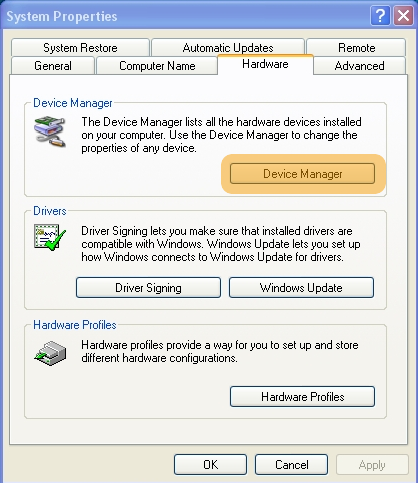
\includegraphics[height=4cm]{images/distance_sensor01.png}
		\label{fig:distance_sensor01.png}
 	}
	\subfigure[]{
		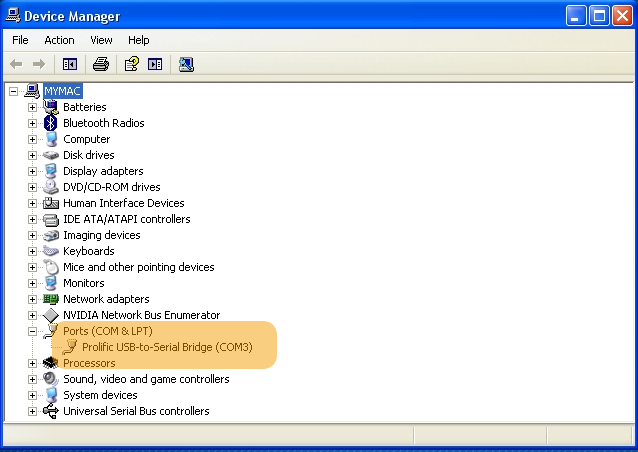
\includegraphics[height=4cm]{images/distance_sensor02.png}
		
 	}
	\caption{Pr�fung, ob nach der Treiberinstallation ein neuer COM-Port angelegt wurde. a) Systemeinstellungsmenu unter Windows, �ffnen des \emph{Device Managers}. b) Es sollte sich ein COM-Port unter dem Men�punkt \emph{Ports (COM\&LPT)} befinden.}
	\label{fig:usbserialadapter}
\end{figure} 

\subsubsection{Testen des Distanzsensors}

Die Software zum Testen des Distanzsensors befindet sich im  Projektverzeichnis um Unterverzeichnis \emph{software/laser\_distance\_sensor}. Die Installation wird �ber \emph{setup.exe} gestartet.

Abbildung \ref{fig:distancesensortest} zeigt, wie die mitgelieferte Software verwendet werden kann, um den Distanzsensor zu testen.

\begin{figure}[ht]
\centering
\subfigure[]{
		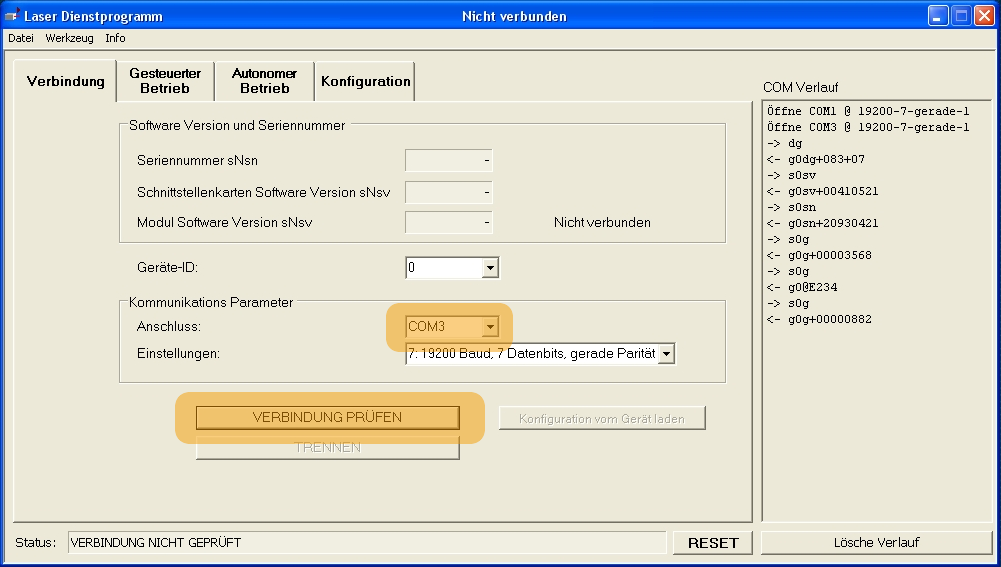
\includegraphics[height=4cm]{images/distance_sensor03.png}
 	}
	\subfigure[]{
		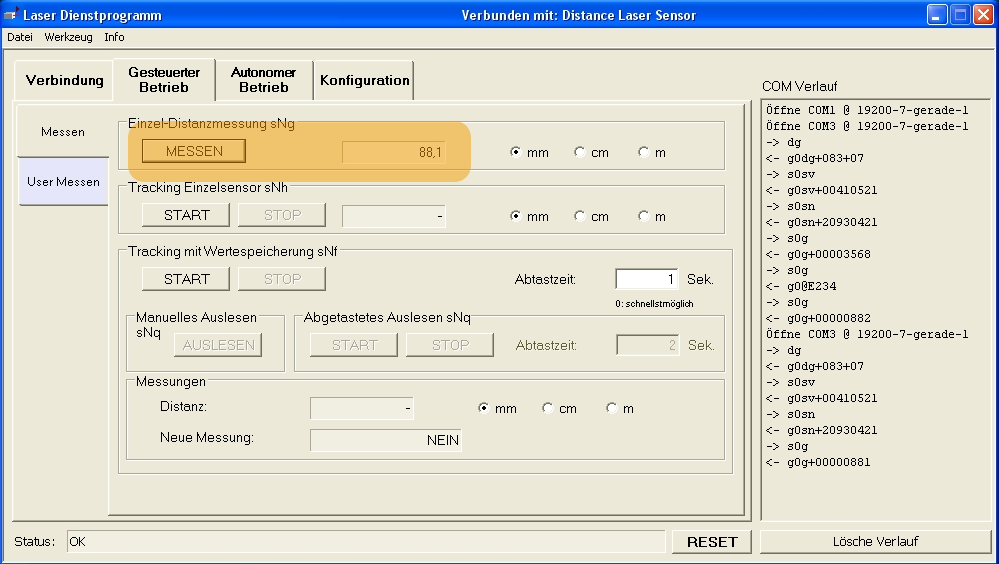
\includegraphics[height=4cm]{images/distance_sensor04.png}
 	}
	\caption{Ausf�hren der installierten Software. a) Auswahl des korrekten COM-Ports und Pr�fen der Verbindung (dabei wird die Verbindung aufgebaut). b) Ausf�hren einer Entfernungsmessung, der gemessene Distanzwert wird direkt angezeigt.}
	\label{fig:distancesensortest}
\end{figure} 